%!TEX root = ../systemnahe-programmierung.tex

\chapter{Entwicklungsumgebung}\label{entwicklungsumgebung}

Zur Entwicklung wird die MCU 8051 \ac{IDE} eingesetzt, welche für Windows und Linux kostenlos zum
Download zur Verfügung steht. Neben den beiden unterstützten Sprachen C und Assemblersprache bietet
die \ac{IDE} einen Simulator um eine Programmierung ohne reele Hardware zu ermöglichen.

\begin{figure}[htbp]
\centering
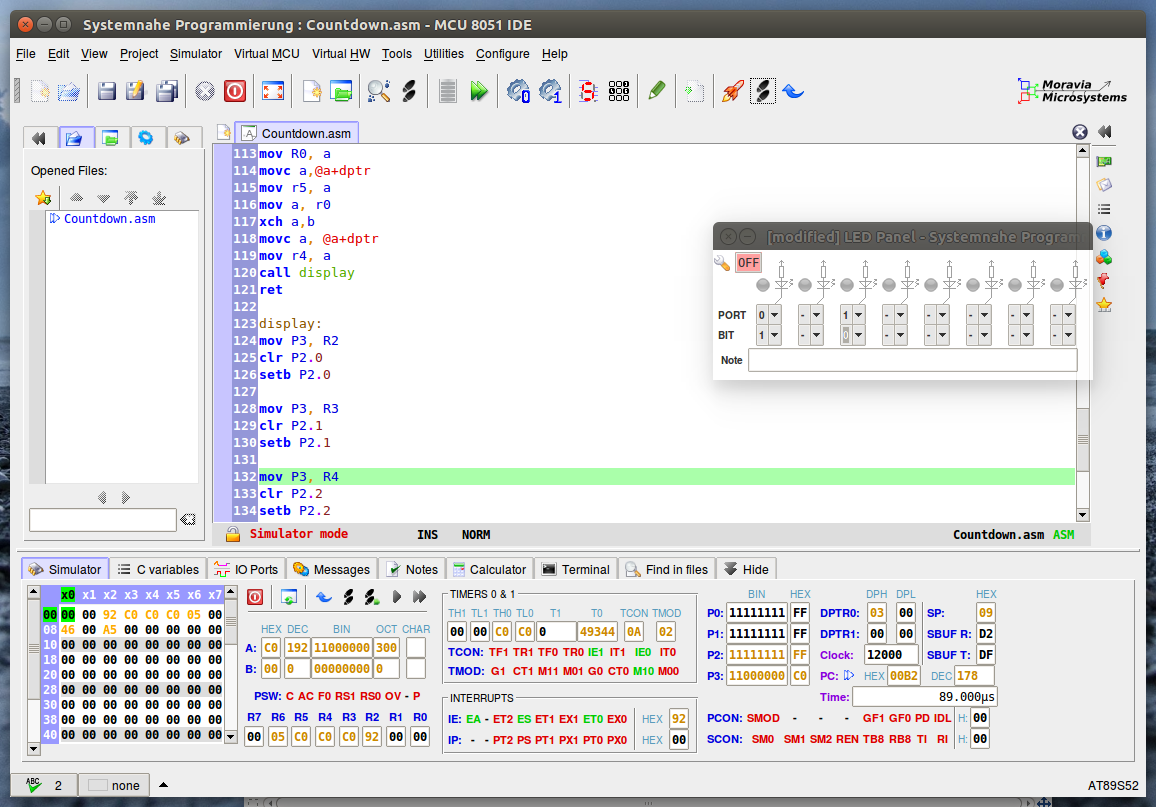
\includegraphics{images/ide.png}
\caption{MCU 8051 IDE}
\end{figure}

Zentrales Element der \ac{IDE} ist der Code Editor, welcher mit üblichen aber auch zusätzlichen
Features aufwartet. Er bietet Funktionen wie Syntax Highlighting, Vervollständigung der Befehle
während des Tippens, Überprüfung der Code Syntax und der Rechtschreibung in Kommentaren. Neben der
Anzeige von Zeilennummern, Lesezeichen und Haltemarken ist es möglich den Code als XHTML oder LaTeX
Dokument zu exportieren.

\begin{figure}[htbp]
\centering
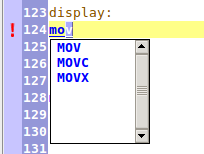
\includegraphics{images/editor.png}
\caption{MCU 8051 IDE Editor}
\end{figure}

Im unteren Bereich der \ac{IDE} ist der Simulator untergebracht. Er virtualisiert einen gewählten
Microcontroller und gibt dem Benutzer die Möglichkeit genau zu erkennen, wie sich die Kompenenten
verhalten, nachdem z.B. der Wert des Registers verändert wird. So wird es möglich bestimmte Fehler
im Programm zu finden, was mit reeler Hardware nahezu unmöglich wäre. Der Benutzer hat darüber
hinaus die Möglichkeit jegliche Speicher zu editieren und das Verhalten direkt zu beobachten. Ein
Abbild des laufenden Programms kann außerdem in einer Datei gespeichert werden und zu einem späteren
Zeitpunkt fortgesetzt werden.

Die \ac{IDE} kann zudem die geöffneten Source Code Dateien samt Konfigurationsparameter in einer
\ac{XML} Datei speichern. Der integrierte wissenschaftliche Rechner bietet unter anderem die
Umrechnung von Zahlen zwischen Hexadezimal, Dezimal, Oktal und Binär Zahlensystemen. Rohdaten können
direkt im integrierten Hexadezimal Editor bearbeitet werden. Assemblercode kann mit dem Disassembler
wieder zurück in Source Code verwandelt werden.

Neben dem Simulator stehen auch eine Zahl an Hardware Visualisierungen zur Verfügung. Mit Hilfe
dieser können \ac{LED}s, Displays oder auch Temperatursensoren an den Simulator angschlossen
werden.\footnote{(o.V.) (o.J.) MCU 8051 IDE, http://www.moravia-microsystems.com/mcu-8051-ide,
  Einsichtnahme: 28.01.2015.}

\begin{figure}[htbp]
\centering
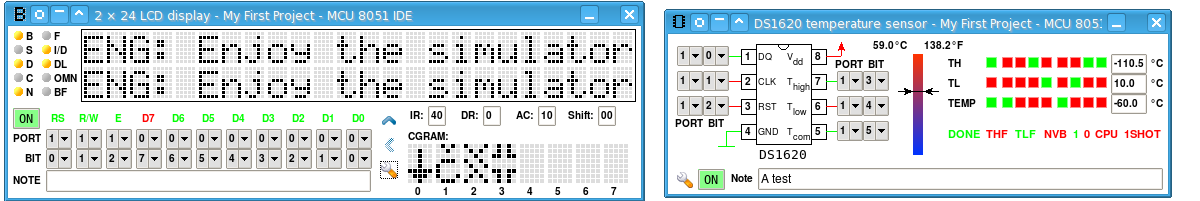
\includegraphics{images/display-temp.png}
\caption{MCU 8051 IDE Hardware Visualisierung}
\end{figure}